% L14a example figure: the three gene network motifs of the example.
%
% Drawn in the style of Shoval and Alon, "SnapShot: Network Motifs", Cell 143
% (2010), doi:10.1016/j.cell.2010.09.050. Each circle is a gene and its protein.
% A blue arrow is activation, and a red line with a flat end is repression.
%   negative autoregulation   X represses its own gene
%   positive autoregulation   X activates its own gene
%   negative feedback loop    X activates Y, and Y represses X
%
% Drawn on November 19, 2026 with the palette and build of the L14a phase
% portrait figure. The notebook SVG carries a dark palette added by theme_svg.py;
% keep new colors in that script's mapping when changing the palette here.
\documentclass[tikz,border=6pt]{standalone}
\usepackage[no-math]{fontspec}
\IfFontExistsTF{Arial}{\setsansfont{Arial}}{\setsansfont{TeX Gyre Heros}}
\renewcommand{\familydefault}{\sfdefault}
\usetikzlibrary{arrows.meta, positioning}

\definecolor{vnink}{HTML}{202124}
\definecolor{gdblue}{HTML}{0091FF}
\definecolor{evred}{HTML}{D93025}
\definecolor{waband}{HTML}{EEF0F2}

\begin{document}
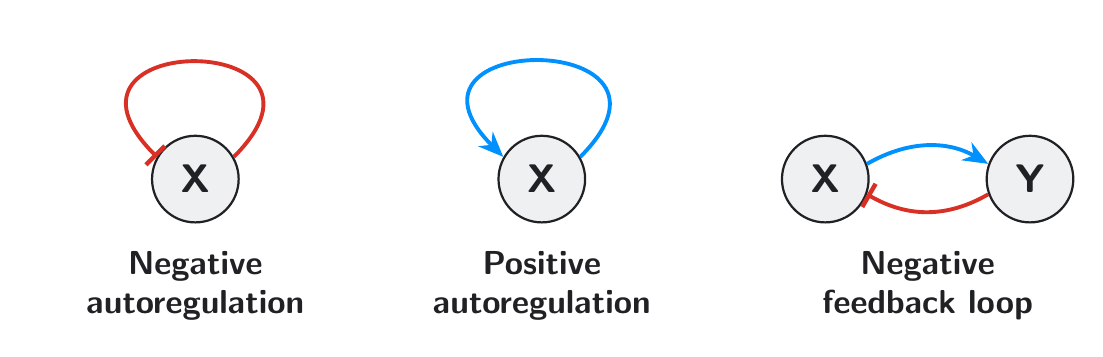
\begin{tikzpicture}[
  font=\sffamily\large,
  gene/.style={circle, draw=vnink, fill=waband, line width=0.8pt, minimum size=1.1cm,
    font=\sffamily\Large\bfseries, text=vnink},
  activates/.style={draw=gdblue, line width=1.4pt, -{Stealth[length=3.2mm, width=2.6mm]}},
  represses/.style={draw=evred, line width=1.4pt, -{Bar[width=3.4mm, line width=1.6pt]}},
  title/.style={font=\sffamily\large\bfseries, text=vnink, align=center},
]

% ------------------------------------------------- negative autoregulation
\node[gene] (nar) at (0, 0) {X};
\draw[represses] (nar.30) to[out=45, in=135, looseness=6] (nar.150);
\node[title] at (0, -1.35) {Negative\\autoregulation};

% ------------------------------------------------- positive autoregulation
\node[gene] (par) at (4.4, 0) {X};
\draw[activates] (par.30) to[out=45, in=135, looseness=6] (par.150);
\node[title] at (4.4, -1.35) {Positive\\autoregulation};

% ------------------------------------------------- negative feedback loop
\node[gene] (x) at (8.0, 0) {X};
\node[gene] (y) at (10.6, 0) {Y};
\draw[activates] (x.20) to[out=30, in=150] (y.160);
\draw[represses] (y.200) to[out=210, in=330] (x.340);
\node[title] at (9.3, -1.35) {Negative\\feedback loop};
\end{tikzpicture}
\end{document}
